\documentclass[11pt]{book}
\usepackage{fontspec}
\setmainfont{TeX Gyre Pagella}
\usepackage[margin=1in]{geometry}
\usepackage{xcolor}
\usepackage{tikz}
\usetikzlibrary{arrows.meta}
\usepackage{amssymb}
\usepackage{enumitem}
\usepackage{titlesec}

\titleformat{\chapter}[display]{\bfseries\Large}{Sproll 02}{0.5em}{\Huge}
\titleformat{\section}{\bfseries\large}{\thesection}{0.6em}{}

\newenvironment{algorithmproc}[1]{%
\vspace{0.6em}\noindent\rule{\linewidth}{0.6pt}\\[0.2em]\textbf{How to Tell: #1}\\[0.3em]}%
{\\[0.2em]\noindent\rule{\linewidth}{0.6pt}\vspace{0.6em}}

\newenvironment{practicenow}{%
\vspace{0.6em}\noindent\rule{\linewidth}{0.6pt}\\[0.2em]\textbf{Practice Now}\\[0.3em]}%
{\\[0.2em]\noindent\rule{\linewidth}{0.6pt}\vspace{0.6em}}

\newenvironment{exercisebox}[1]{%
\vspace{0.8em}\noindent\rule{\linewidth}{0.6pt}\\[0.2em]\textbf{Exercises: #1}\\[0.3em]%
\begin{enumerate}[label=\arabic*., itemsep=0.4em]}%
{\end{enumerate}\noindent\rule{\linewidth}{0.6pt}\vspace{0.6em}}

\newenvironment{trythis}{%
\vspace{0.6em}\noindent\rule{\linewidth}{0.6pt}\\[0.2em]\textbf{Try This}\\[0.3em]}%
{\\[0.2em]\noindent\rule{\linewidth}{0.6pt}\vspace{0.6em}}

\newenvironment{summarybox}{%
\vspace{0.6em}\noindent\rule{\linewidth}{0.6pt}\\[0.2em]\textbf{What We Learned}\\[0.3em]}%
{\\[0.2em]\noindent\rule{\linewidth}{0.6pt}\vspace{0.6em}}

\begin{document}
\begin{titlepage}
\centering
\vspace*{1.4in}
{\Huge \textbf{SPROLL 02}}\\[0.5in]
{\huge What Happened First?}\\[0.8in]
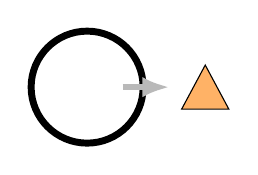
\begin{tikzpicture}
\draw[line width=2.5pt] (-1,0) circle (0.28in);
\draw[fill=orange!60] (0.2,-0.28) -- (0.5,0.28) -- (0.8,-0.28) -- cycle;
\draw[-{Latex[length=3.5mm]}, line width=2pt, gray!55] (-0.55,0) -- (0.05,0);
\end{tikzpicture}\\[0.8in]
{\Large The Sproll Curriculum}\\[0.2in]
{\large Cycle I: Pops --- Things, Differences, and Counting}
\end{titlepage}

\tableofcontents

\chapter*{Before You Begin}
\addcontentsline{toc}{chapter}{Before You Begin}

Sproll 01 introduced the Pop, the act of choosing one thing out of several possible things, and showed that a sequence of Pops builds up a history. It also showed that you can count how many Pops happened. This workbook asks a question Sproll 01 never quite settled: once two Pops have happened, does the order they happened in leave any trace you could find later, just by looking at the result?

The honest answer, worked out carefully in this workbook, is: sometimes yes, and sometimes surprisingly no. That surprise is the whole point of this book.

\chapter{Two Choices, One After Another}

\section{Building a History Step by Step}

Suppose you choose the circle first, from a field of three shapes, and afterward you choose the triangle, from a second, separate field of three shapes.

\begin{center}
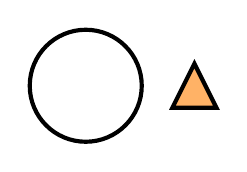
\begin{tikzpicture}
\draw[line width=1.5pt] (-0.7,0) circle (0.28in);
\draw[fill=orange!60, line width=1.5pt] (0.4,-0.28) -- (0.68,0.28) -- (0.96,-0.28) -- cycle;
\end{tikzpicture}
\end{center}

Two Pops happened, in this order: circle, then triangle. Here is what the picture looks like once both choices have been made. Notice that the picture itself does not show any arrows, timestamps, or numbers telling you which shape arrived first. It just shows a circle and a triangle, sitting there.

Turning on lights in a room works the same way. Imagine you switch on a lamp on your desk, and a little while later you switch on the overhead light too. Once both lights are on, anyone who walks into the room afterward simply sees a room with two lights on. Nothing about the room itself announces which light was switched on first.

\begin{algorithmproc}{What a Finished Picture Shows}
A finished picture, or a room, or any result you can look at after several choices have already been made, shows you what is currently true. It does not automatically show you the order in which those things became true. Whether the order can be recovered at all is a separate question, taken up later in this workbook.
\end{algorithmproc}

\begin{practicenow}
Pick two choices you could make in either order, for example, putting on a jacket and putting on a hat, or watering one plant and then another. Do them in one order and look at the result. Would a person who walked in only at the end be able to tell which one you did first, just from looking?
\end{practicenow}

\begin{exercisebox}{Section 1.1}
\item Describe, in your own words, the difference between ``two Pops happened'' and ``two Pops happened in a particular order.''
\item Think of an everyday result (a made bed, a set table, a finished puzzle) where the order of the steps that produced it is genuinely impossible to tell just by looking at the result. Describe it.
\item Think of a different everyday result where the order actually is still visible somehow, even after everything is finished. Describe it, and explain what makes it different from your answer to the previous question.
\end{exercisebox}

\chapter{Starting Over, a Different Order}

\section{The Same Two Shapes, the Other Way Around}

Now start completely over, with a fresh field of three shapes, choose the triangle first, and choose the circle second.

\begin{center}
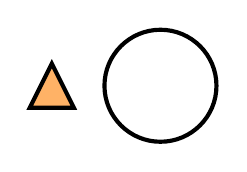
\begin{tikzpicture}
\draw[line width=1.5pt] (0.7,0) circle (0.28in);
\draw[fill=orange!60, line width=1.5pt] (-0.4,-0.28) -- (-0.68,0.28) -- (-0.96,-0.28) -- cycle;
\end{tikzpicture}
\end{center}

Compare this picture to the one from Chapter 1. They show exactly the same two shapes, in exactly the same arrangement. If someone handed you both pictures without telling you anything else, you would have no way to tell that one of them was built circle-first and the other triangle-first. As far as the pictures alone are concerned, the two histories are indistinguishable.

The lights example makes this even clearer. If you had instead switched on the overhead light first and the desk lamp second, the finished room, both lights on, looks exactly like the room from the earlier example. Two genuinely different sequences of events, switching lamp then overhead, or overhead then lamp, produced the exact same final result.

\begin{algorithmproc}{Comparing Two Endings}
To check whether two results are ``the same,'' first ask what you are actually comparing them by. If you are comparing only the finished picture, or only the current state of the room, two genuinely different histories can easily produce identical results. Being identical in that comparison does not mean the two histories themselves were identical; it only means that particular way of comparing them could not tell them apart.
\end{algorithmproc}

\begin{trythis}
Pack a small bag with two items, in one order. Empty it, and pack it again with the same two items, in the opposite order. Does the bag look any different at the end, depending on the order you packed it in? What if you used items of very different sizes, so one had to go in first to fit?
\end{trythis}

\begin{exercisebox}{Section 2.1}
\item In the lights example, explain in your own words why ``lamp first, then overhead'' and ``overhead first, then lamp'' can end in the exact same result.
\item Describe a situation similar to your Try This exercise, where the order of packing or building something genuinely does change the final appearance, even though the same objects are involved either way.
\item Challenge: come up with your own pair of choices, made in two different orders, where you predict the final result will look identical either way. Test your prediction if you can.
\end{exercisebox}

\chapter{What a Picture Remembers and What It Forgets}

\section{The Question the Picture Cannot Answer}

Here is the puzzle this workbook has been building toward. Look again at the circle-and-triangle picture. It is genuinely impossible to tell, from the picture alone, whether the history that produced it was circle-then-triangle or triangle-then-circle. Both histories are completely real, completely different from each other, and yet they collapse into one indistinguishable picture once you are only looking at the final result.

This does not mean the order never mattered, or that the two histories were secretly the same thing all along. It means a picture is a kind of summary, and summaries can throw information away. A librarian who only sees which books are currently checked out cannot tell you the order in which they were checked out. A cook who only tastes the finished soup cannot always tell which spice went in first. In each case, something real happened in a particular order, and the final result, on its own, does not preserve that order.

\begin{algorithmproc}{Does the Order Matter Here?}
Before assuming a final result tells you the whole story, ask whether the way you are looking at it, a taste, a photograph, a tally, was built to preserve order in the first place. Some ways of looking at something do keep track of order (a numbered list, a diary with dates, a video recording). Others do not (a single photograph of a finished scene, a simple count of objects, a taste). The same real history can look completely different depending only on which kind of look you take at it.
\end{algorithmproc}

\section{Keeping a Record on Purpose}

If a finished picture cannot answer the question, something else has to. Imagine keeping a written record as each choice happens, instead of only looking at the result afterward: a small list, in order, of exactly what was chosen and when.

\begin{center}
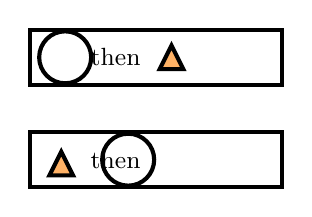
\begin{tikzpicture}
\draw[line width=1.5pt] (-1.6,0.55) rectangle (1.6,1.25);
\draw[line width=1.5pt] (-1.15,0.9) circle (0.13in);
\node[right] at (-0.95,0.9) {\small then};
\draw[fill=orange!60, line width=1.5pt] (0.05,0.75) -- (0.2,1.05) -- (0.35,0.75) -- cycle;
\draw[line width=1.5pt] (-1.6,-0.75) rectangle (1.6,-0.05);
\draw[fill=orange!60, line width=1.5pt] (-1.35,-0.6) -- (-1.2,-0.3) -- (-1.05,-0.6) -- cycle;
\node[right] at (-0.95,-0.4) {\small then};
\draw[line width=1.5pt] (-0.35,-0.4) circle (0.13in);
\end{tikzpicture}
\end{center}

The two strips above record the two histories from this workbook exactly, one shape at a time, in the order each one was chosen. Unlike the finished pictures, these two records look nothing alike: the top one clearly reads circle-then-triangle, and the bottom one clearly reads triangle-then-circle. A record kept in order, on purpose, can answer exactly the question a finished picture cannot.

\begin{summarybox}
Two genuinely different histories can produce the exact same finished picture, because a finished picture is a summary, and summaries can leave out the order in which things happened. A record kept deliberately, in order, as events happen, can recover exactly what a finished picture leaves out. Same things. Different history.
\end{summarybox}

\begin{exercisebox}{Section 3.1}
\item Explain, in your own words, why a written, in-order record can tell histories apart that a finished picture cannot.
\item Think of a real record-keeping tool people use in everyday life specifically because a finished result would not preserve enough information on its own (examples: a receipt, a sign-in sheet, a browser history). Explain what information it preserves that a simple end result would lose.
\item Challenge: is it possible for even a written record to lose some information about order, if it is not detailed enough? Describe a record that keeps track of some order but not all of it.
\end{exercisebox}

\chapter*{Looking Ahead}
\addcontentsline{toc}{chapter}{Looking Ahead}

This workbook showed that a kept record, unlike a finished picture, can answer the ``what happened first'' question. But that raises a new question of its own. If a record is only useful because it claims to show what really happened, how would you ever check whether it can be trusted? Could you take a record and actually rebuild, step by step, the exact sequence of events it describes, to see whether doing so gives you back the same result every time?

That question is the subject of the next workbook, Sproll 03: Play It Again.

\chapter*{For Parents and Teachers}
\addcontentsline{toc}{chapter}{For Parents and Teachers}

This workbook's central content is a genuine mathematical limitation, not a simplification chosen for a young reader: recovering the order of events from a result alone is not always possible, and whether it is possible depends entirely on how the result was produced from the underlying history, not on the history itself. The two full example histories used throughout this book (circle-then-triangle and triangle-then-circle) are constructed as two independent sequences, each starting fresh, rather than as two branches from one shared choice point; this sidesteps a formal complication (branching histories sharing a common prefix) that a more advanced treatment would need to handle explicitly, and that this curriculum takes up in later, more technical material.

Chapter 3's distinction between a finished picture and a kept record anticipates a precise idea developed later in this curriculum: that a single history can be observed in more than one way, and different ways of observing it can either preserve or discard specific information, such as order. This workbook does not name that idea formally; it only makes sure the child has felt the surprise of it directly; namely, that ``looks the same'' is not the same claim as ``happened the same way,'' before any formal vocabulary is attached to the distinction.

\end{document}
